\section{Packet counts}
\label{s:PacketCounts}

While examining the numbers, there are a few numbers that break out of the scope of each timing template.
Those who really point out the numbers in the table are the service discovery scan used with an insane and aggressive timing template and the ping scan used with an aggressive and normal timing template.
Nmap, by default, uses the normal timing template ($-T3$) to conduct scanning activities \autocite{10.5555/1538595}.
In table \ref{tbl:PacketPrSecond} the packets pr. the second rate has many similarities to the given timing template compared to other types of scans.
However, there are some numbers that stands out such as the \textit{ping scan} using the \textit{aggressive} and \textit{normal} timing template, and the service scan using \textit{insane} and \textit{aggressive} timing template. These numbers are significantly higher compared to the other scans in the table with the corresponding timing template. 
In the \textit{insane} column the packet per second rate is mainly between 1216 and 1559, \textit{aggressive} between 1195 and 1732 and \textit{normal} between 1196 and 1566 packets per second.



\begin{table}[htbp]
\caption{Measurement of packets pr. second}
\begin{center}
\begin{tabular}{|r|r|r|r|r|r|r|}
\hline
\textbf{Nmap scan}&\textbf{insane}&\textbf{aggressive}&\textbf{normal}&\textbf{polite}&\textbf{sneaky}&\textbf{paranoid}\\
\hline
xmas scan&1310.072&1229.611&1196.482&49.980&1.333&0.067\\
\hline
fin scan&1328.788&1195.168&1296.515&49.978&1.333&0.067\\
\hline
null scan&1310.763&1288.222&1309.800&49.980&1.333&0.067\\
\hline
ping scan&1216.341&2477.556&2104.646&49.936&1.333&0.067\\
\hline
tcp full scan&1559.437&1732.328&1566.229&50.004&1.335&0.067\\
\hline
service scan&3348.940&4072.136&1253.609&49.979&1.333&0.067\\
\hline
\end{tabular}
\label{tbl:PacketPrSecond}
\end{center}
\end{table}

Another interesting packet per second finding is the \textit{service discovery scan}, which used significantly more time in the \textit{insane} and \textit{aggressive} scan compared to other scan types.
This clearly also points toward a commonly used type of scan where the user would want a fast reply, therefore using either the \textit{insane} or \textit{aggressive} timing template to quickly retrieve a scan result.
Figure \ref{fig:PngNorHist} confirms these findings, though 9 of the ten normal ping scans are shown to be in the range of 53ms (milliseconds) and 164ms. The \nth{10} scan in comparison used 326ms, which used significantly more time than the other scans, and this increases the average duration time significantly.
Within figure \ref{fig:PngAgrHist} the aggressive ping scan shows similar results where 9 out of 10 scans used between 54ms and 152ms where the \nth{10} scan took 590ms. Within this scan, the average scan duration time is increased due to this \nth{10} scan.
Similar to these findings is the insane service discovery scan shown in figure \ref{fig:SvcInsHist} and the aggressive service discovery scan shown in figure \ref{fig:SvcAgrHist}.
The insane service discovery scan had nine scans which took between 56ms and 216ms, where the \nth{10} took 915ms, as shown in figure \ref{fig:SvcInsHist}.
9 out of the ten aggressive service discovery scans used between 54ms and 107ms, shown in figure \ref{fig:SvcAgrHist}, where the \nth{10} took over 13 times the time (1.44 seconds) that next on the list did. This can point to a high network load when conducting a certain number of scans from one scanner host.

\vfill
\clearpage

\newpage
\vfill
\begin{figure}[!ht]%
    \centering
    \subfloat[ping scan insane\label{fig:PngInsHist}]{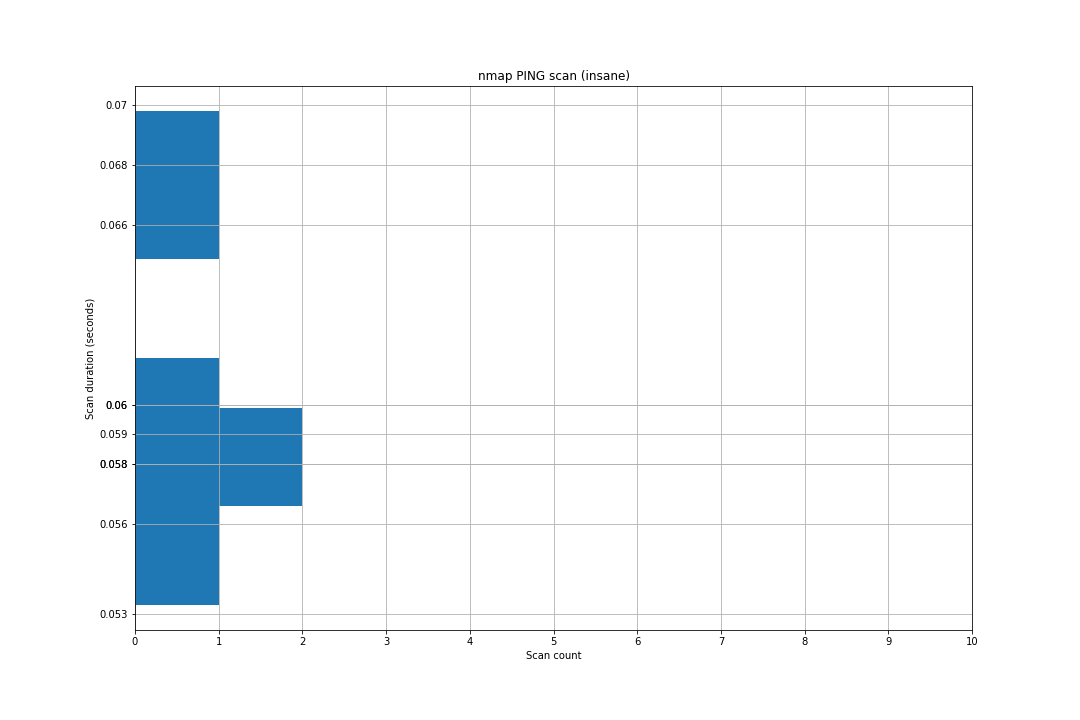
\includegraphics[width=8.3cm]{images/analysis/pingscan/insane/Histogram.png}}
    \subfloat[ping scan aggressive\label{fig:PngAgrHist}]{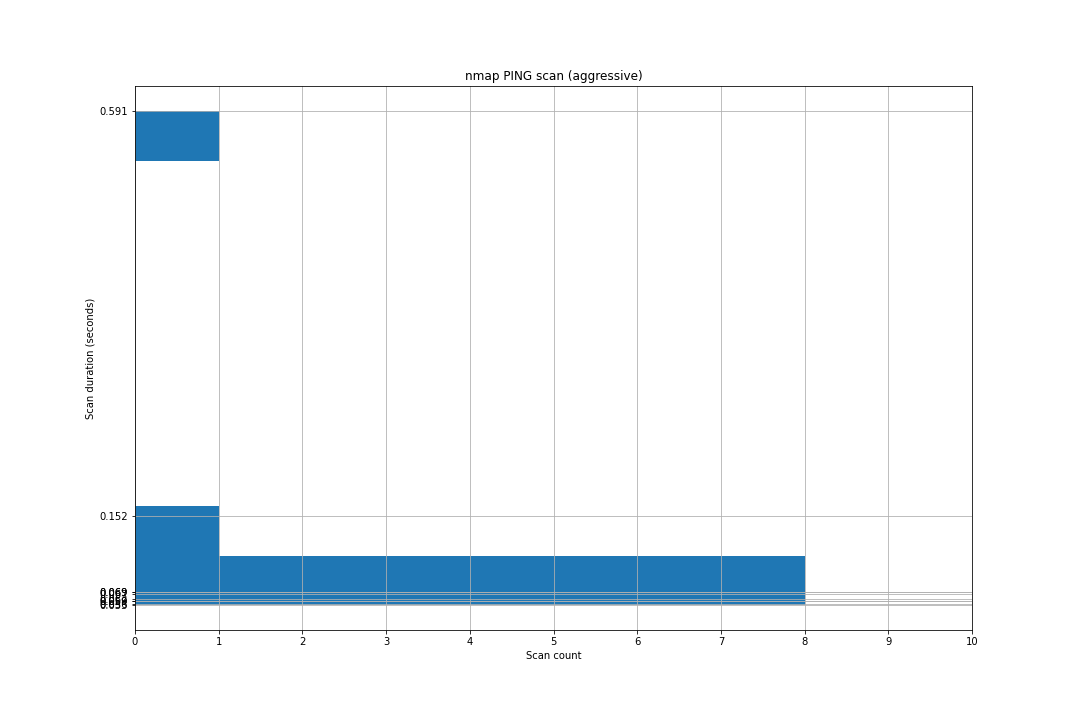
\includegraphics[width=8.3cm]{images/analysis/pingscan/aggressive/Histogram.png}} \\
    \subfloat[ping scan normal\label{fig:PngNorHist}]{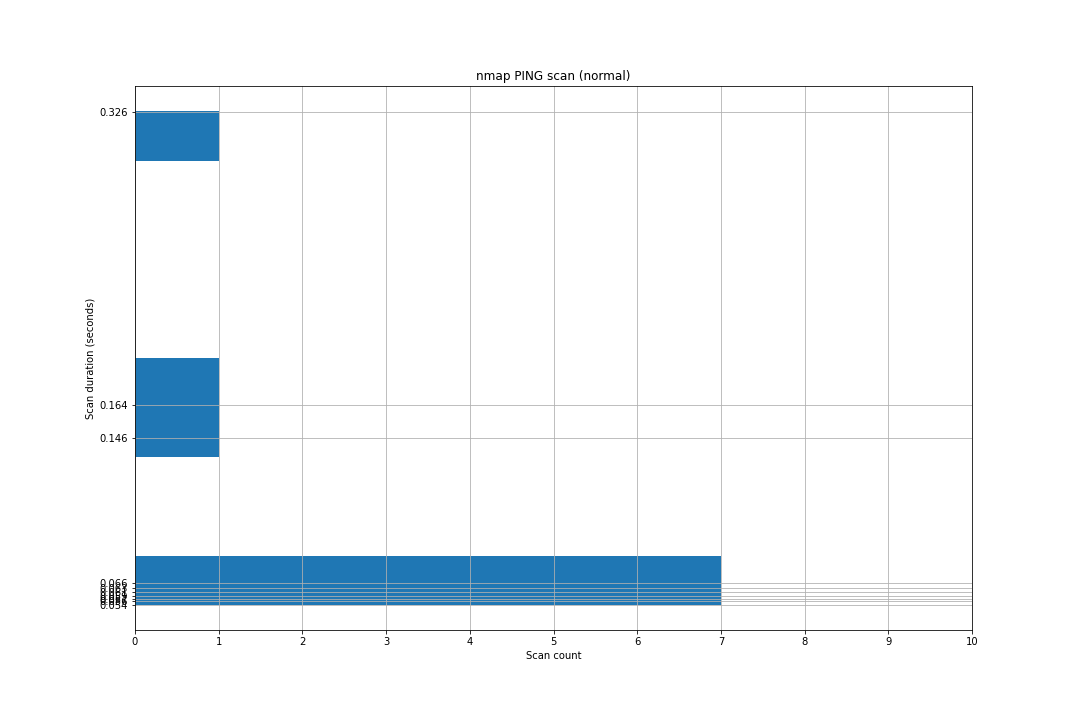
\includegraphics[width=8.3cm]{images/analysis/pingscan/normal/Histogram.png}}
    \subfloat[service discovery insane\label{fig:SvcInsHist}]{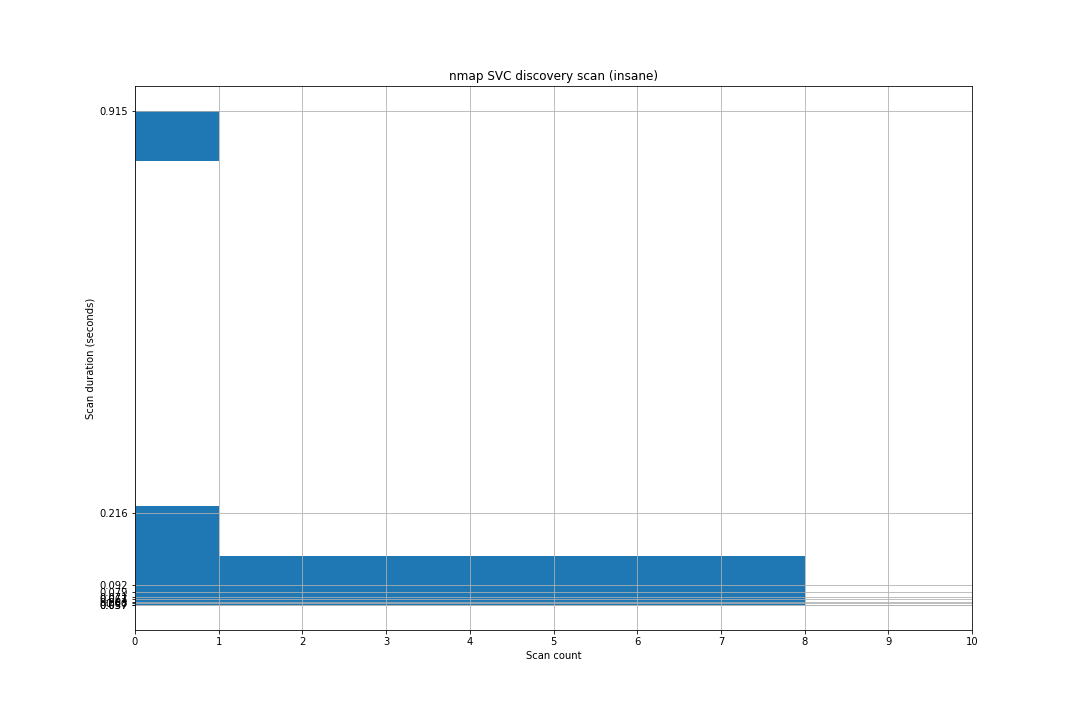
\includegraphics[width=8.3cm]{images/analysis/svcscan/insane/Histogram.png}} \\
    \subfloat[service discovery aggressive\label{fig:SvcAgrHist}]{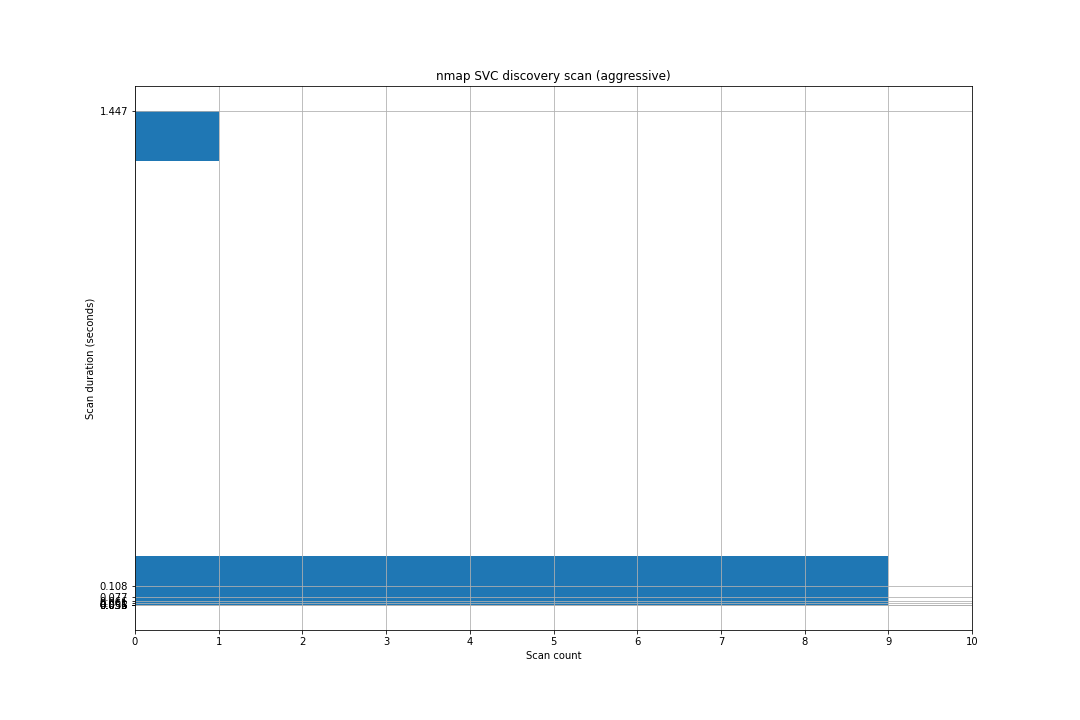
\includegraphics[width=8.3cm]{images/analysis/svcscan/aggressive/Histogram.png}}
    \subfloat[service discovery normal\label{fig:SvcNorHist}]{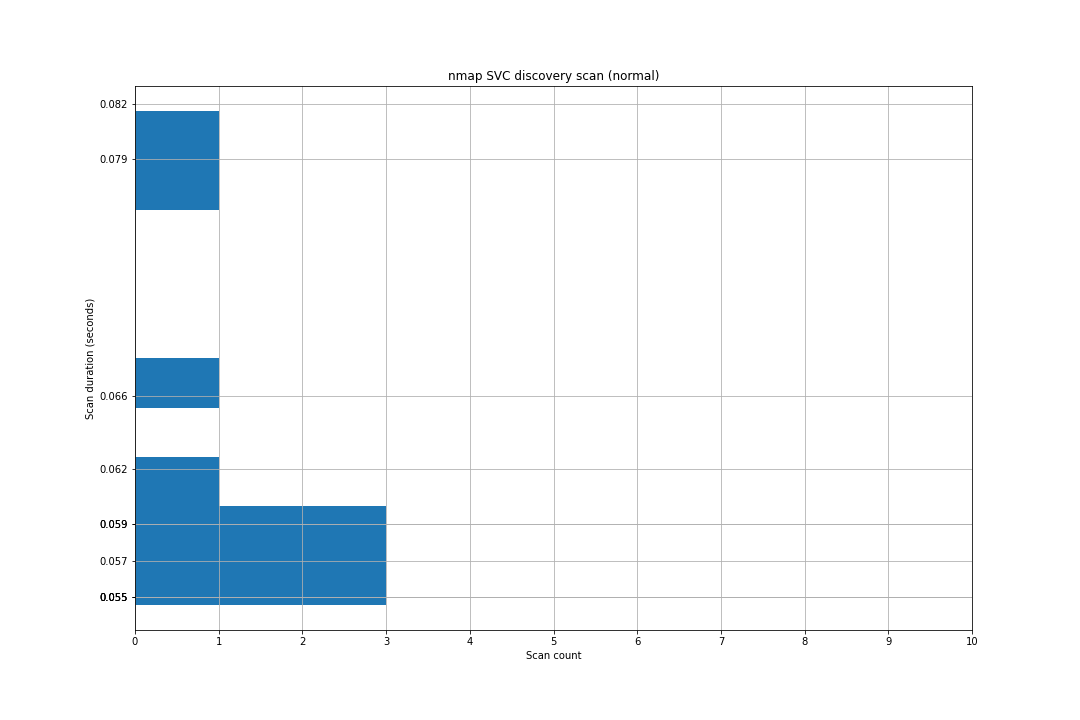
\includegraphics[width=8.3cm]{images/analysis/svcscan/normal/Histogram.png}}
    \caption{Identifying scans significantly increasing scan duration}
    \label{fig:PingSvcInsAgrNormHist}%
\end{figure}

\begin{table}[htbp]
\caption{Description of scan duration standing out statistics (seconds)}
%\ref{tbl:StandOutScanDuration}
\begin{center}

\begin{tabular}{|r|r|r|r|r|r|r|}
\hline
&svc insane&svc aggressive&ping normal&ping aggressive&ping insane&svc normal\\
\hline
count&10&10&10&10&10&10\\
\hline
mean&0.167&0.204&0.105&0.124&0.061&0.063\\
\hline
std&0.267&0.437&0.087&0.166&0.005&0.010\\
\hline
min&0.057&0.055&0.054&0.055&0.053&0.055\\
\hline
25\%&0.060&0.056&0.057&0.059&0.058&0.055\\
\hline
50\%&0.069&0.058&0.062&0.064&0.059&0.059\\
\hline
75\%&0.089&0.074&0.126&0.069&0.064&0.065\\
\hline
max&0.915&1.447&0.326&0.591&0.070&0.082\\
\hline
\end{tabular}
\label{tbl:StandOutScanDuration}
\end{center}
\end{table}

The scan metrics for these scans are merged into table \ref{tbl:StandOutScanDuration} where also a collection of two other scans, shown in figure \ref{fig:PngInsHist} and figure \ref{fig:SvcNorHist}, are located.
These two scans, the insane ping scan and the normal service discovery scan, show a very small standard deviation ($std$) as low as $0.005$ seconds (5ms) and $0.010$ seconds (10ms). This shows signs of the normal time a scan of the given type with the given timing template would take. In comparison, the other four scans have a significantly higher standard deviation, where the highest is the aggressive service discovery has a standard deviation of 437ms.
The deviation results for the insane ping scan and normal service discovery scan prove a normal scan with a decent deviation.

As presented in table \ref{tbl:StandOutScanDuration}, only a chosen collection of scan types and timing templates are presented. These are in detail described in each respective Jupyter notebook in appendix \ref{app:ElectronicResources}.
